\section*{Informations générales}
 
\begin{table}[H]
\centering
	\begin{tabularx}{16.8cm}{|X|X|}
	\hline
	\rowcolor{gray!40} Numéro du risque & Type du risque \\
	\hline
	001 & Crash du serveur \\
	\hline
	\end{tabularx}
\end{table}

\begin{table}[H]
\centering
	\begin{tabularx}{16.8cm}{|X|X|X|}
	\hline
	\rowcolor{gray!40} Date & Visa du \RQ & Visa du \CP \\
	\hline
	 07/12/15 & pgpic & pgpic \\
	\hline
	\end{tabularx}
\end{table}

\begin{table}[H]
\centering
	\begin{tabularx}{16.8cm}{|X|X|X|X|}
	\hline
	\rowcolor{gray!40} Pilote & Activité WBS & Compte WBS & Phase d'apparition \\
	\hline
	 \Matthieu & Suivre les Risques et Opportunités & 1.2.3.2 & À partir de l’installation serveur\\
	\hline
	\end{tabularx}
\end{table}

\section*{Description du risque}

\subsection*{Résumé}
	Le risque lié au crash du serveur peut entraîner la perte de toutes les données et l'impossibilité d'utiliser le service mis en place.
	
\subsection*{Analyse des causes}
	voir figure.

\subsection*{Criticité}

\begin{table}[H]
\centering
	\begin{tabularx}{16.8cm}{|>{\columncolor{gray!40}}X|X|}
	\hline
	Gravité & 4\\
	\hline
	Probabilité & 1\\
	\hline
	Criticité & Critique\\
	\hline
	\end{tabularx}
\end{table}
\newpage

\section*{Actions}
\subsection*{Actions préventives}

%\begin{table}[H]
\centering
	\begin{longtable}{|p{7cm}|p{7cm}|}
	\hline
	\rowcolor{gray!40} Numéro de cause & Actions préventives \\
	\hline
	 1 & \begin{itemize}
	 	\item Boîte à idée
	 	\item Faire des tickets
	 	\item Réunions fréquentes
	 	\item Laisser la parole à tout le monde
	 	\item Hiérarchie bien définie
	 	\item Choisir les bons outils
	 	\item Faire des compte rendus de réunion à envoyer au client
	 	\item Être en constante délibération
	 	\item Reformulation des spécifications
	 	\item Avoir un interlocuteur unique entre le client et le \PICCourt
	 	\item Suivi hebdomadaire de l'avancement
	 \end{itemize} \\
	\hline
	2 & \\
	\hline
	3 & \begin{itemize}
		\item Choisir de bonnes valeurs seuils
		\item Présence et assiduité
		\item Créneau horaire respecté
		\item Objectifs personnels
	\end{itemize} \\
	\hline
	4 & \begin{itemize}
		\item La personne qui fait les tests doit être différente de celle qui code
		\item Faire un maximum de tests
		\item Définir clairement les méthodes de travail dès le début du \PICCourt et faire vérifier par un référent
	\end{itemize} \\
	\hline
	5 & \begin{itemize}
		\item Se former sur la réalisation d'un audit sécurité
		\item Effectuer régulièrement des audits sécurité
		\item Nommer un responsable sécurité
		\item Faire des tests en boîte noire et boîte blanche
	\end{itemize} \\
	\hline
	6 & \begin{itemize}
		\item Faire les démarches nécessaires
		\item Être économe
		\item Faire un calcul du budget au début
	\end{itemize} \\
	\hline
	7 & \begin{itemize}
		\item Faire un planning
		\item Faire un GANTT/PERT
		\item Chacun respecte son rôle
		\item Bien définir les rôles
		\item Faire des réunions fréquentes
		\item Utiliser les bons outils de partage
	\end{itemize} \\
	\hline
	8 & \begin{itemize}
		\item Avoir une méthode de paiement de secours
		\item Se renseigner auprès des prestataires
		\item Demander au département les méthodes de paiement autorisées
	\end{itemize} \\
	\hline
	9 & \begin{itemize}
		\item Former un bénévole
	\end{itemize} \\
	\hline
	10 & \begin{itemize}
		\item Actions de prévention et de formation
		\item Effectuer des sauvegardes régulières
	\end{itemize} \\
	\hline
	\end{longtable}
%\end{table}

\subsection*{Plan de contournement}

\begin{enumerate}
	\item Bloquer le site
	\item Demander un serveur temporaire
	\item Faire les démarches nécessaires pour les réparations
	\item Relancer le site
\end{enumerate}

\section*{Décision de clôture}
Par le \CP{} et le pilote du risque.
\begin{table}[H]
\centering
	\begin{tabularx}{16.8cm}{|X|X|}
	\hline
	\rowcolor{gray!40} Date de clôture & Raison de la clôture \\
	\hline
	  & \\
	\hline
	\end{tabularx}
\end{table}

\section*{Historique des modifications}
\begin{table}[H]
\centering
	\begin{tabularx}{16.8cm}{|X|X|}
	\hline
	Date & Modification \\
	\hline
	  & \\
	\hline
	\end{tabularx}
\end{table}
\newpage

\begin{landscape}
\begin{figure}
	\centering
	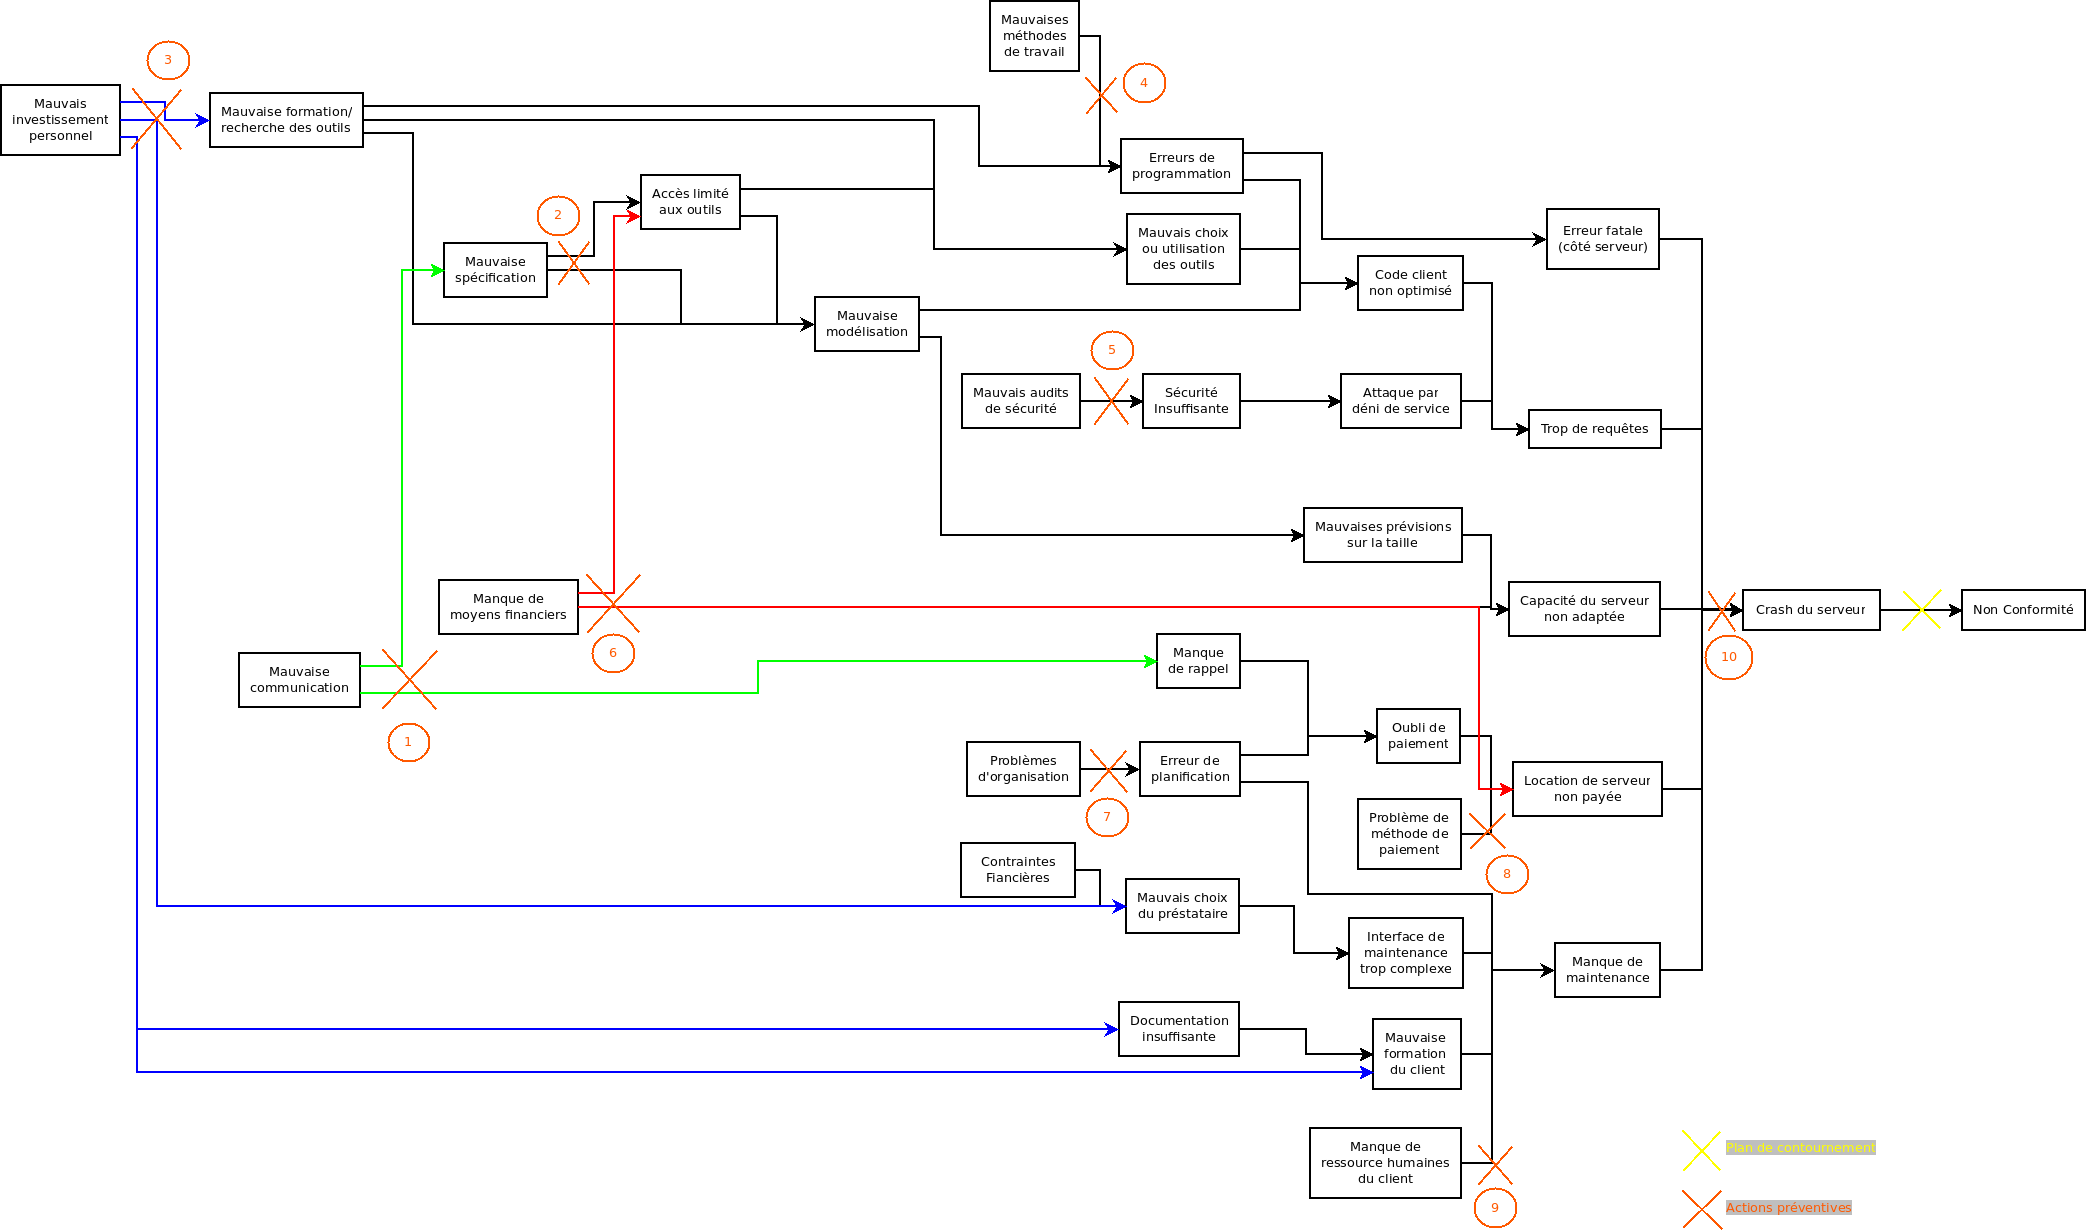
\includegraphics[scale=0.35]{images/AnalyseRisque_nPourquoi.png}
\end{figure}
\end{landscape}